\section{Simulation Analysis}

Using the ngspice program, we began by analysing the circuit for $t<0$, the currents and voltages at each node are summarized in the table below.

%%%%%INCLUDE TABLE 
\begin{table}[h]
  \centering
  \begin{tabular}{|l|r|}
    \hline    
    {\bf Name} & {\bf Value [A or V]} \\ \hline
    @r1[i] & -2.58478e-04\\ \hline
@r2[i] & 2.705006e-04\\ \hline
@r3[i] & -1.20225e-05\\ \hline
@r4[i] & -1.17739e-03\\ \hline
@r5[i] & 2.705006e-04\\ \hline
@r6[i] & 9.189098e-04\\ \hline
@r7[i] & 9.189098e-04\\ \hline
@c[i] & 0.000000e+00\\ \hline
v(1) & 5.134559e+00\\ \hline
v(2) & 4.871563e+00\\ \hline
v(3) & 4.321260e+00\\ \hline
v(4) & -1.87652e+00\\ \hline
v(5) & 4.908647e+00\\ \hline
v(6) & 5.722227e+00\\ \hline
v(7) & -1.87652e+00\\ \hline
v(8) & -2.80082e+00\\ \hline

  \end{tabular}
  \caption{Operating point. A variable preceded by @ is of type {\em current}
    and expressed in mA; other variables are of type {\it voltage} and expressed in
    Volt.}
  \label{tab:op1}
\end{table}

Then we proceeded to calculate the tensions $V_6$ and $V_8$, for time $t=0s$, with an applied tension of $0V$, and where the capacitor was substituted by a independent voltage source which imposes a voltage equal to $V_6-V_8$. This is indeed, necessary to establish the boundary conditions for the system, for $t>0s$, since in the instant $t=0s$ the applied tension is $0v$, thus by performing the operating point analyses for the conditions described above, the initial values of the aforementioned tensions may be obtained. The capacitor is replaced by a voltage source because at that instant for our purposes the tension at each of its terminals is constant since we are holding time still.
The results that were obtained are shown bellow


%%%%%INCLUDE TABLE 
\begin{table}[h]
  \centering
  \begin{tabular}{|l|r|}
    \hline    
    {\bf Name} & {\bf Value [A or V]} \\ \hline
    @r1[i] & -2.58478e-04\\ \hline
@r2[i] & 2.705006e-04\\ \hline
@r3[i] & -1.20225e-05\\ \hline
@r4[i] & -1.17739e-03\\ \hline
@r5[i] & 2.705006e-04\\ \hline
@r6[i] & 9.189098e-04\\ \hline
@r7[i] & 9.189098e-04\\ \hline
@c[i] & 0.000000e+00\\ \hline
v(1) & 5.134559e+00\\ \hline
v(2) & 4.871563e+00\\ \hline
v(3) & 4.321260e+00\\ \hline
v(4) & -1.87652e+00\\ \hline
v(5) & 4.908647e+00\\ \hline
v(6) & 5.722227e+00\\ \hline
v(7) & -1.87652e+00\\ \hline
v(8) & -2.80082e+00\\ \hline

  \end{tabular}
  \caption{Operating point for $V_s = 0$V and  $t = 0$s. A variable preceded by @ is of type {\em current}
    and expressed in mA; other variables are of type {\it voltage} and expressed in
    Volt.}
  \label{tab:op1}
\end{table}


Using the results listed above, we then simulated the natural response of the circuit, imposing that the initial voltage at node 6 be equal to what we obtained beforehand. To accomplish it, we set the independent voltage source to $0V$ and ,as was expected, the capacitor discharged, following a negative exponential model, as is shown 

%%%%%INCLUDE BONECO DA SOLUÇÃO NATURAL
\begin{figure}[h] \centering
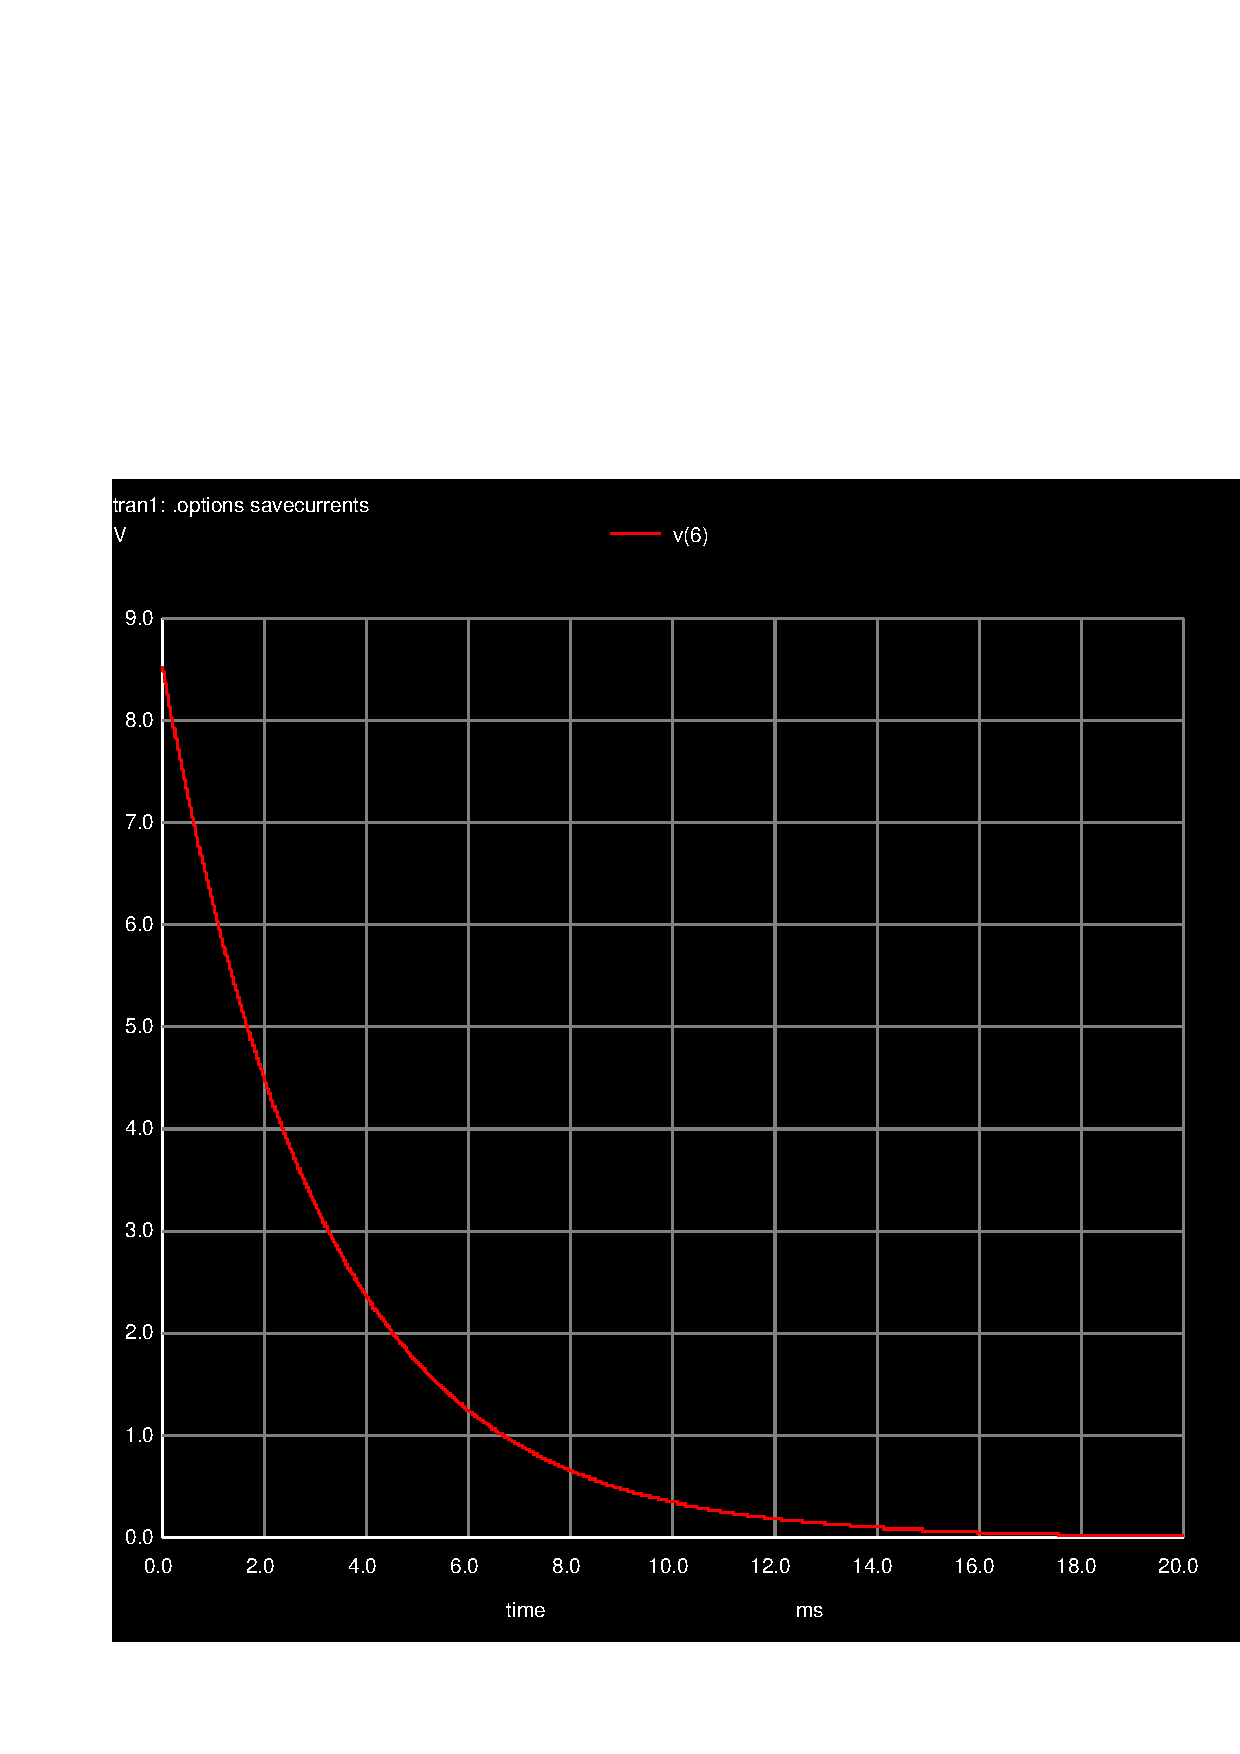
\includegraphics[width=0.6\linewidth]{../sim/3/trans.pdf}
\caption{Natural solution for $t > 0$ s}
\label{fig:Natural solution}
\end{figure}

We then, repeated the same process but this time for the general solution, consisting on the natural and the forced solutions, with the same initial conditions as before. We expected to observe a sinusoidal signal of the same frequency of the applied tension, supper imposed with the previous exponential solution, which as we can see was obtained 


%%%%%INCLUDE BONECO DA SOLUÇÃO GERAL
\begin{figure}[h] \centering
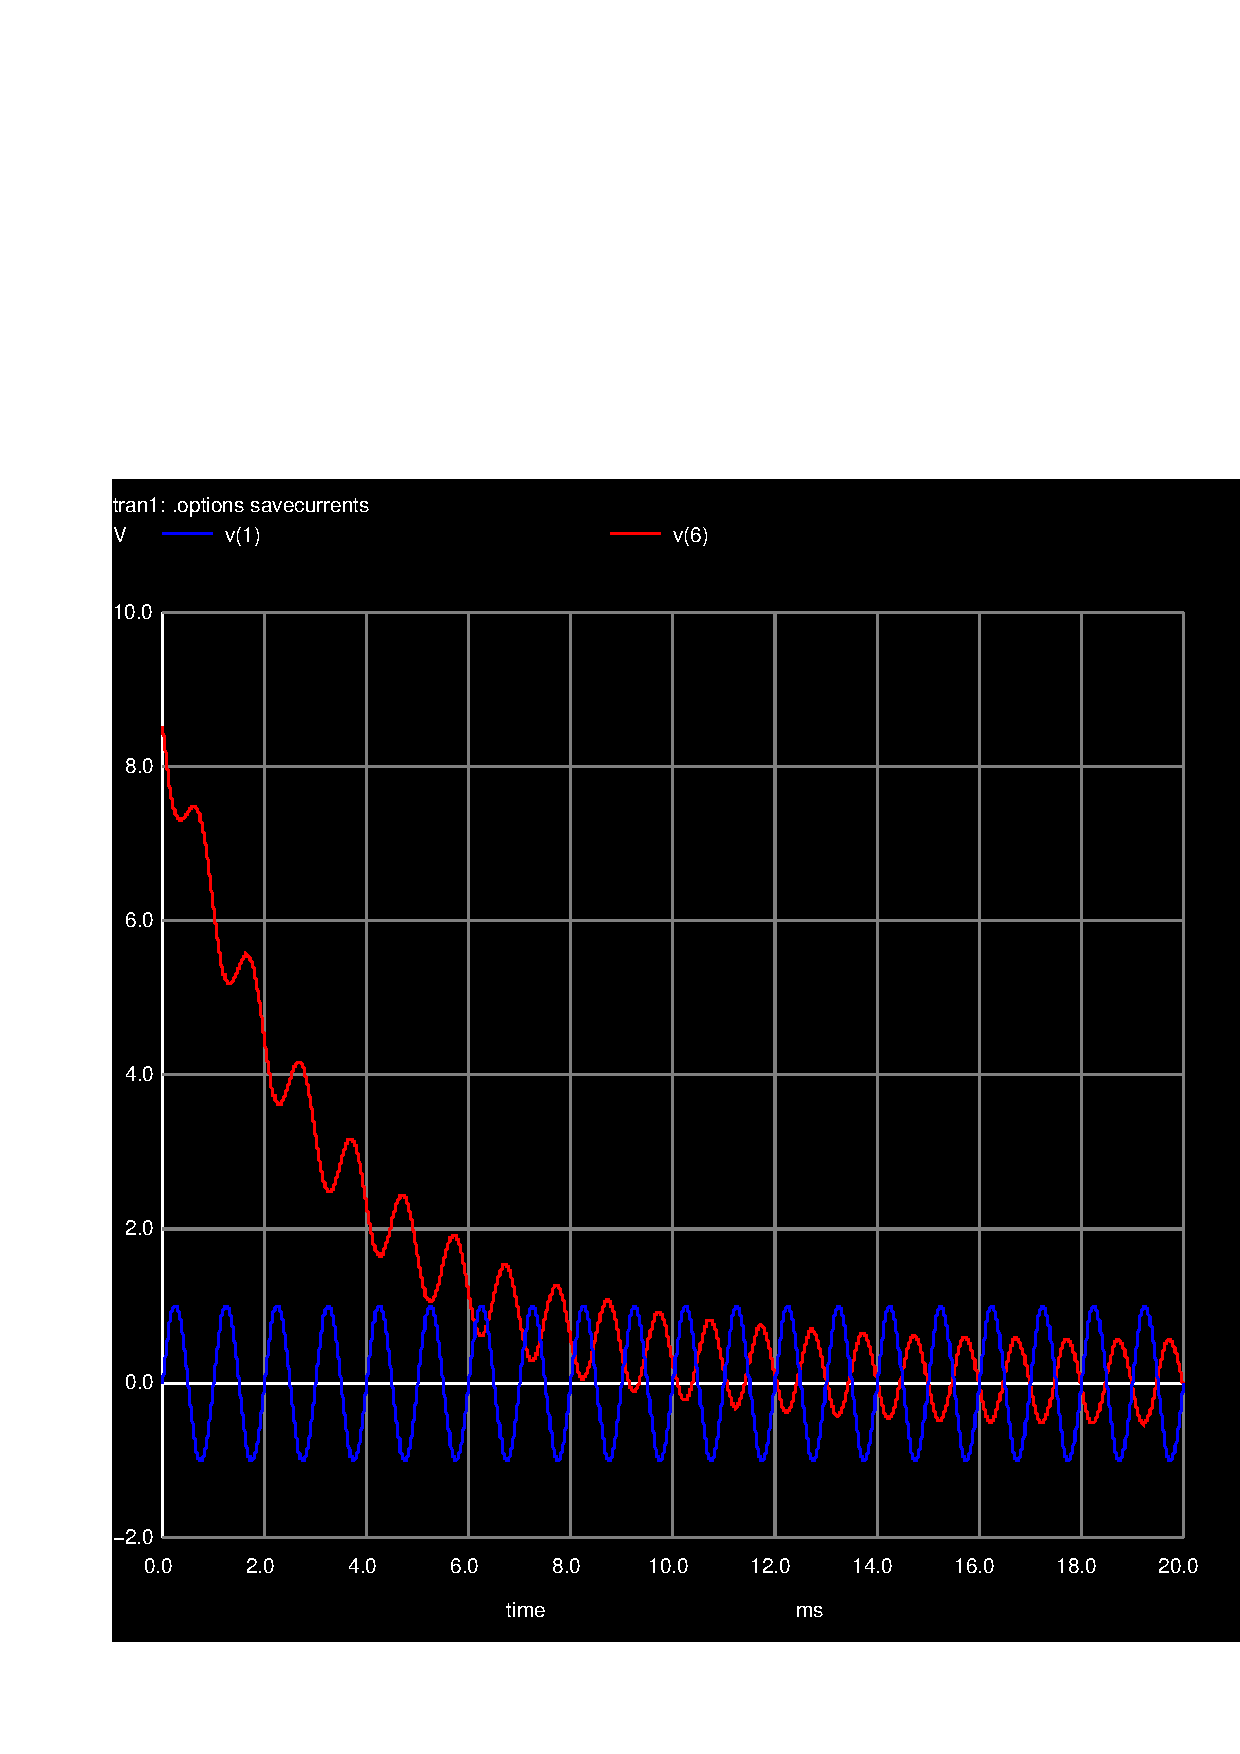
\includegraphics[width=0.6\linewidth]{../sim/4/trans.pdf}
\caption{Full solution for $t > 0$ s}
\label{fig:Full solution}
\end{figure}

At last, we simulated the systems response to several different driving frequencies ranging from 0.1Hz to 1MHz, and the resultant magnitude and phase of the ensuing voltages ($V_6,V_S,V_C$) where plotted, the first the magnitude was expressed in decibels, the second in degrees, and in both cases the x scale is logarithmic. The graphs obtained follow


%%%%%INCLUDE BONECO DA FASE E ÂNGULO
\begin{figure}[h] \centering
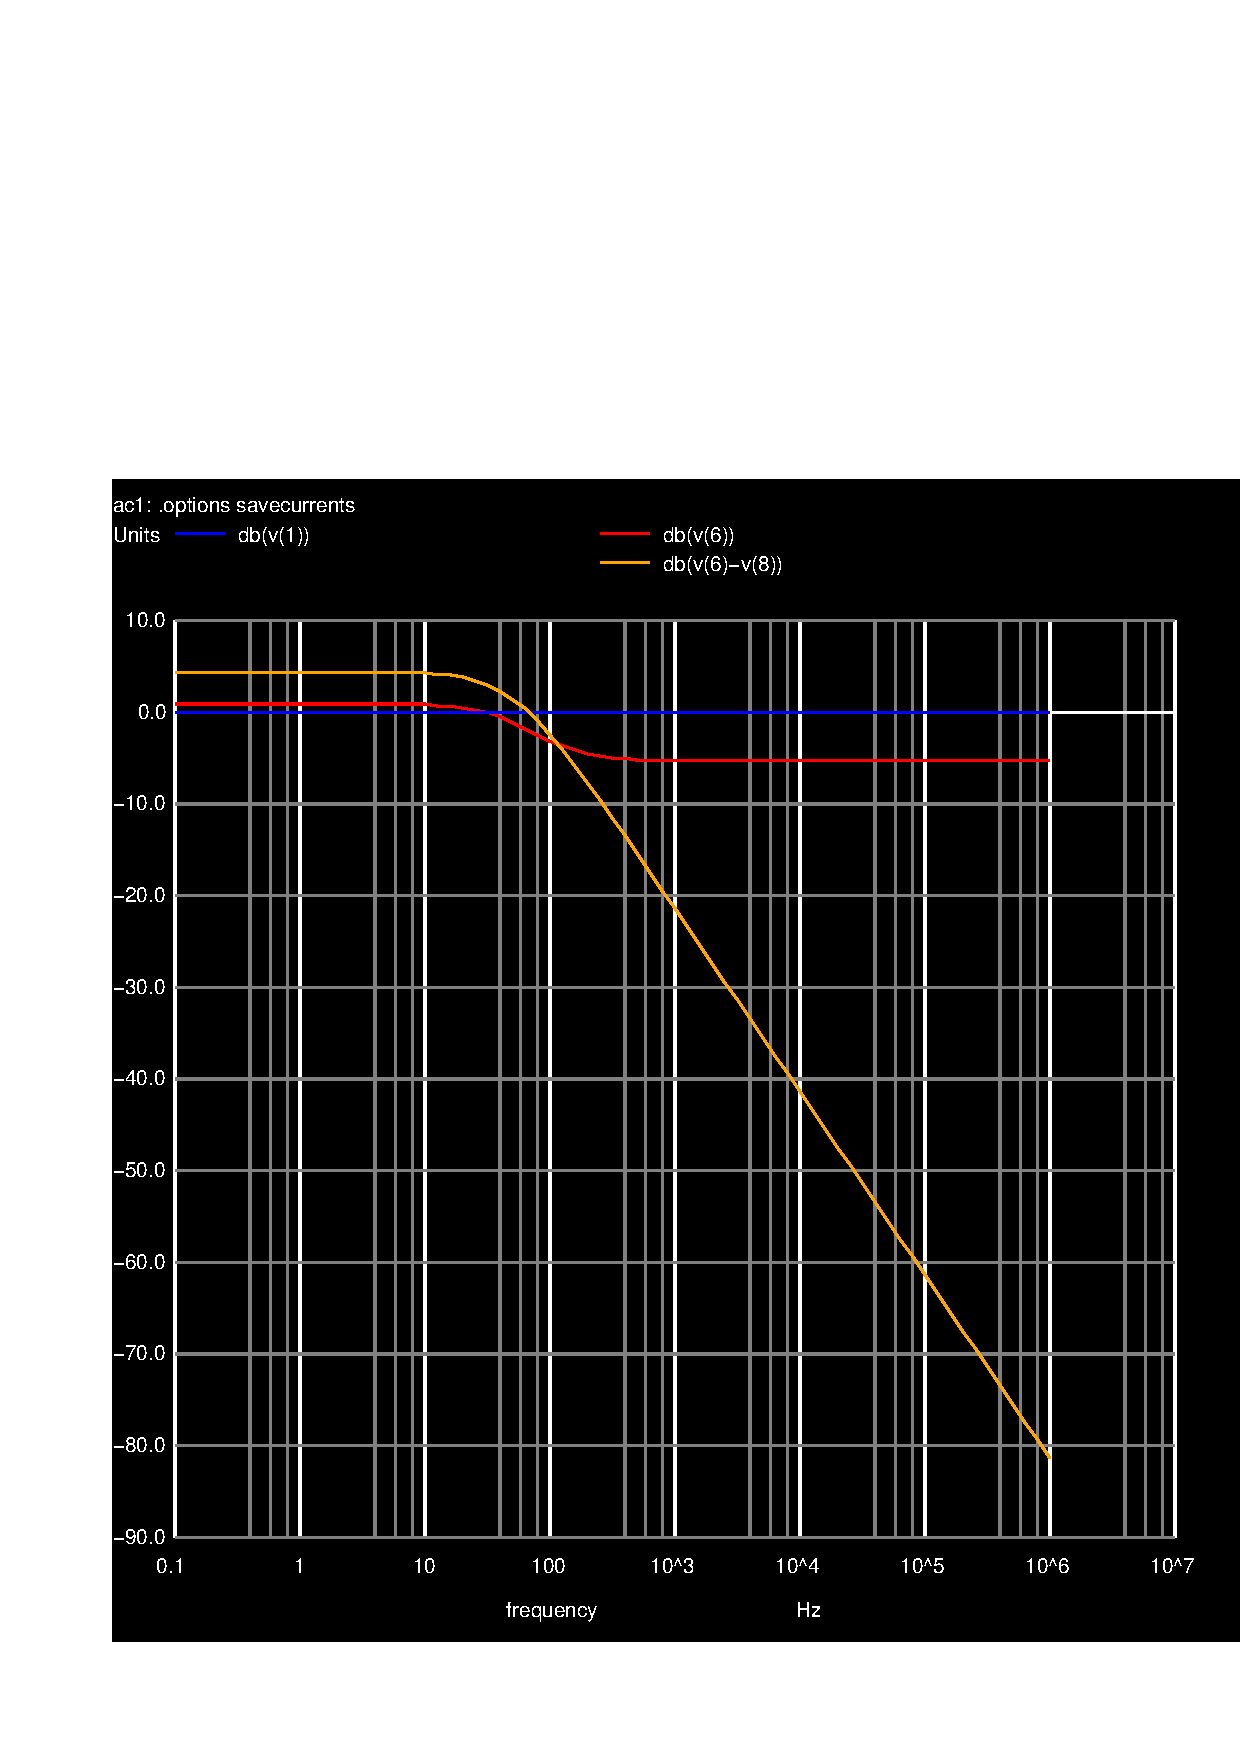
\includegraphics[width=0.6\linewidth]{../sim/5/acm.pdf}
\caption{Circuit's amplitude response}
\label{fig:Amp response}
\end{figure}

\begin{figure}[h] \centering
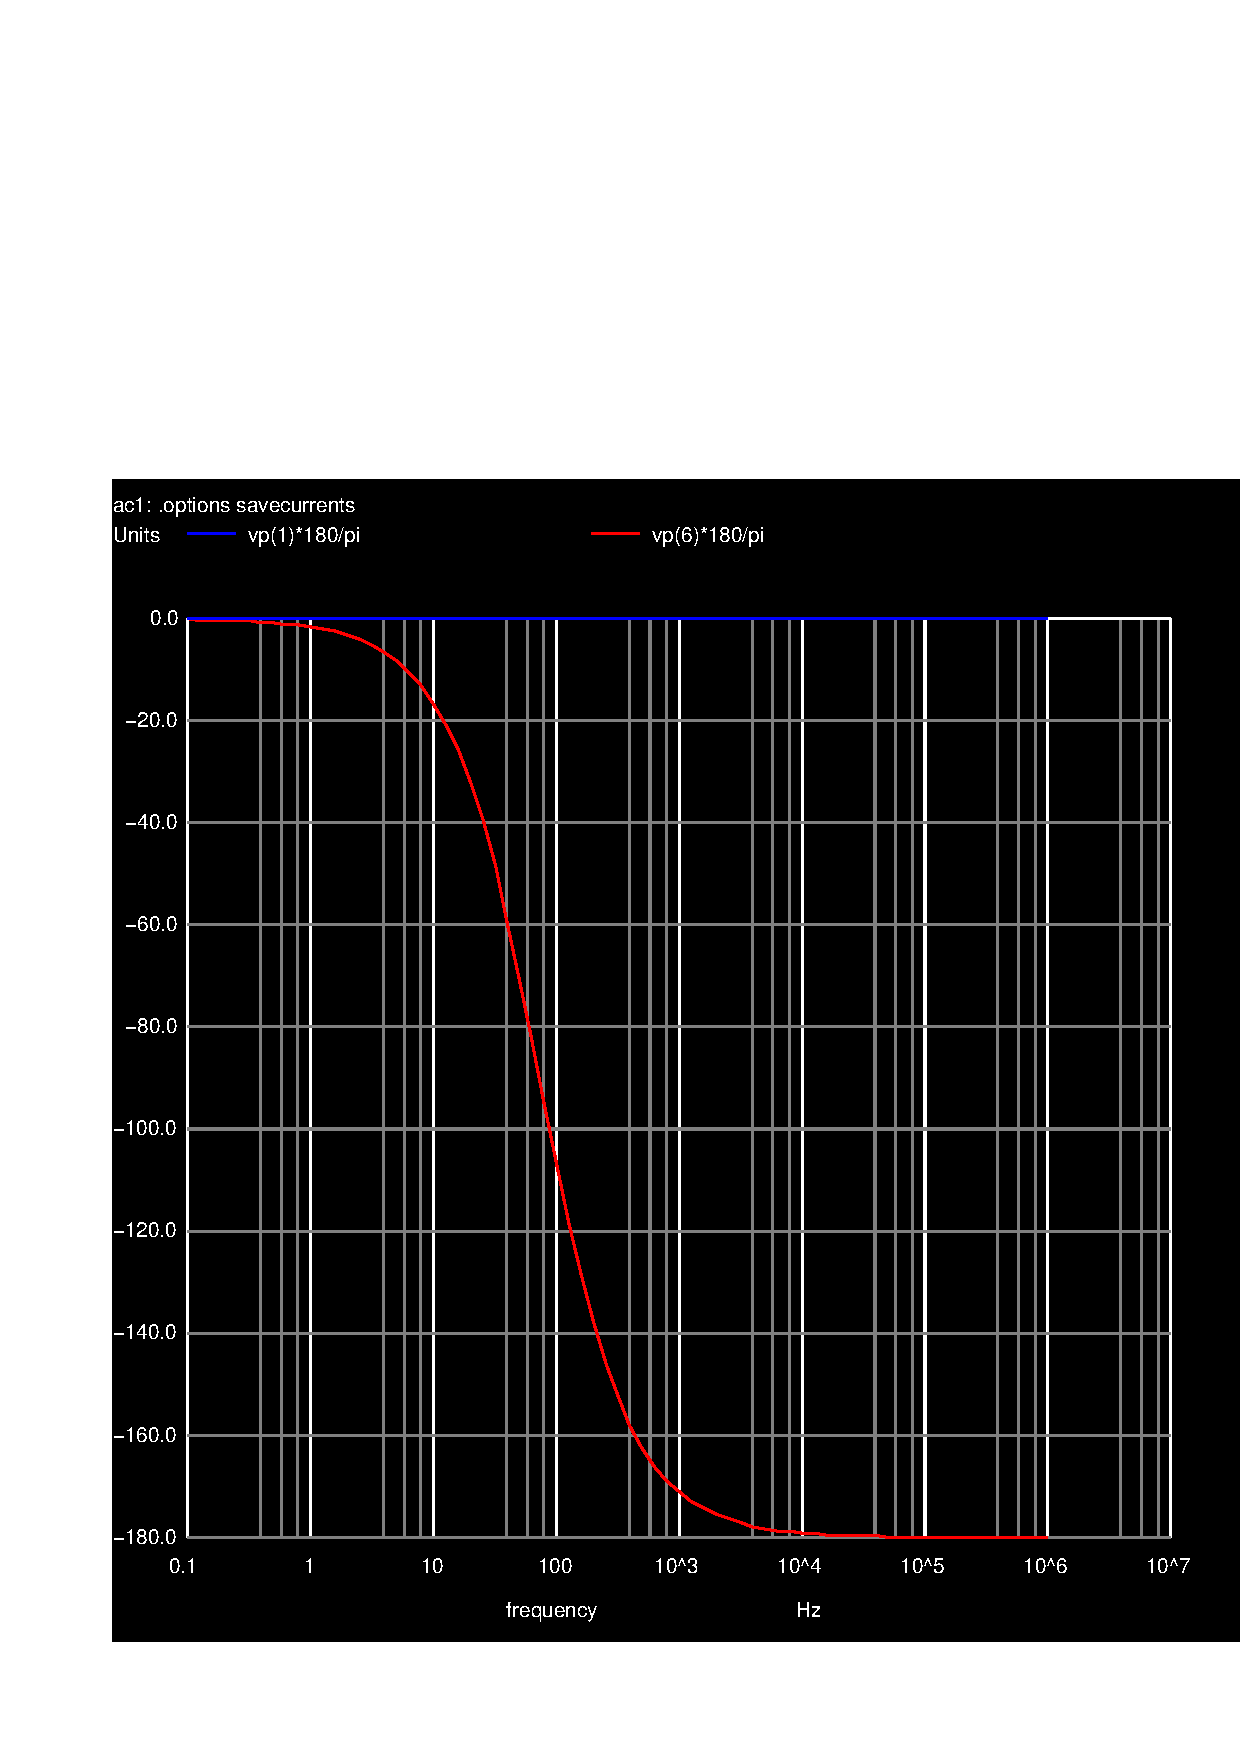
\includegraphics[width=0.6\linewidth]{../sim/5/freq.pdf}
\caption{Circuit's phase response}
\label{fig:Phase response}
\end{figure}







